\chapter{生物的多样化}\label{ch:g12:diversification-of-life}

面包小麦有 42 条\omterm{def:g11:cell-cycle-mitosis:chromosome}{染色体}，分为六组，每组七条：它是
三种野生禾草杂交而成，杂交发生了两次，地点在最早农民的田间。
一条蟒蛇有三百块椎骨，一只小鼠只有三十块，然而
它们用相同的\omterm{def:g10:universal-dna:gene}{基因}构建脊柱。岩石上的地衣是
两种生物，一种真菌和一种藻类，它们长期合为一体，
以至于两者都已无法单独存在。一只年幼的黑猩猩通过观察母亲，学会了用石头
砸开坚果，这发生在一片森林中，那里
一百千米外的黑猩猩从未学会此法。\omterm{def:g11:mutations:mutation}{突变}与上一章的\omterm{def:g10:universal-dna:gene}{基因}重组，
并不是生物产生差异的唯一途径；
本章将介绍其他途径。

\section{不止于突变}

\begin{proposition}[多样化的来源]\label{prop:g12:diversification-of-life:sources}
点\omterm{def:g11:mutations:mutation}{突变}和有性生殖中的\omterm{def:g10:universal-dna:gene}{基因}重组产生了新的\omterm{def:g10:universal-dna:gene}{等位基因}，
以及它们的新组合。除此之外，生物的多样性还由
在更大尺度上改变\omterm{def:g10:universal-dna:gene}{基因}组的过程所产生：
\omterm{def:g10:universal-dna:gene}{基因}复制、从其他\omterm{def:g10:biodiversity-scales:species}{物种}导入\omterm{def:g10:universal-dna:gene}{基因}、增加整套\omterm{def:g11:cell-cycle-mitosis:chromosome}{染色体}——
以及在发育过程中改变现有\omterm{def:g10:universal-dna:gene}{基因}的使用方式，
\omterm{def:g10:biodiversity-scales:species}{物种}间的关联，以及在动物中，通过
完全不依赖\omterm{def:g10:universal-dna:gene}{基因}的行为传递。
\end{proposition}
\admitted

\section{由旧基因产生新基因}

\begin{proposition}[基因复制与分化]\label{prop:g12:diversification-of-life:duplication}
不等\omterm{prop:g12:meiosis-genetic-shuffling:crossingover}{交叉互换}（见\cref{ch:g12:meiosis-genetic-shuffling}）或
复制错误可能使一条\omterm{def:g11:cell-cycle-mitosis:chromosome}{染色体}上保留某个\omterm{def:g10:universal-dna:gene}{基因}的两个拷贝。其中一个
拷贝继续执行原有功能；另一个则摆脱了这一约束，
积累\omterm{def:g11:mutations:mutation}{突变}，并可能获得新功能——也可能丢失。
经过长期演化重复此过程，便产生了\emph{基因家族}\index{基因家族}：
由同一祖先演化而来的一组相关\omterm{def:g10:universal-dna:gene}{基因}，其相似程度
记录了复制发生的先后顺序。
\end{proposition}
\begin{proof}[证据]
\cref{ch:g11:the-eye}中的三种\omterm{def:g11:the-eye:photoreceptors}{视蛋白}和视紫红质构成一个这样的家族；
另一个是珠蛋白家族：编码血红蛋白各条链的若干\omterm{def:g10:universal-dna:gene}{基因}，
血红蛋白——一个用于胚胎，一个用于胎儿，两个用于
成体——以及肌红蛋白\omterm{def:g10:universal-dna:gene}{基因}，即肌肉中储存氧气的蛋白，
成簇位于两条\omterm{def:g11:cell-cycle-mitosis:chromosome}{染色体}上，序列同一性为 40\% 至 80\%，
它们的系统树与\omterm{def:g10:common-ancestry:bodyplan}{脊椎动物}类群出现的先后顺序一致。
\omterm{def:g10:universal-dna:gene}{基因}组中携带数百个这样的家族，
而且每个\omterm{def:g10:universal-dna:gene}{基因}组中都有相当大的一部分由重复片段构成。
\end{proof}

\begin{omfigure}
\begin{tikzpicture}[font=\small, line cap=round, >=Stealth]
  \tikzset{g/.style={draw, fill=omDef!30, minimum height=0.45cm, minimum width=1.2cm, inner sep=1pt, font=\scriptsize}}
  % step 1: one gene
  \draw[thick] (0,3) -- (4,3); \node[g] at (2,3) {珠蛋白};
  \node[anchor=east] at (-0.2,3) {祖先基因};
  \draw[->, thick] (2,2.65) -- (2,2.15) node[midway, right] {复制};
  % step 2: two identical copies
  \draw[thick] (0,1.8) -- (5.4,1.8); \node[g] at (1.6,1.8) {珠蛋白}; \node[g] at (3.4,1.8) {珠蛋白};
  \node[anchor=east] at (-0.2,1.8) {两个拷贝};
  \draw[->, thick] (2.5,1.45) -- (2.5,0.95) node[midway, right] {各自积累突变};
  % step 3: diverged
  \draw[thick] (0,0.6) -- (5.4,0.6); \node[g, fill=omThm!30] at (1.6,0.6) {$\alpha$-珠蛋白}; \node[g, fill=omMeth!30] at (3.4,0.6) {$\beta$-珠蛋白};
  \node[anchor=east] at (-0.2,0.6) {两个基因};
  \draw[->, thick] (2.5,0.25) -- (2.5,-0.25) node[midway, right] {进一步复制};
  \draw[thick] (0,-0.6) -- (7.6,-0.6);
  \node[g, fill=omThm!30] at (1.0,-0.6) {$\zeta$}; \node[g, fill=omThm!30] at (2.4,-0.6) {$\alpha$};
  \node[g, fill=omMeth!30] at (4.2,-0.6) {$\varepsilon$}; \node[g, fill=omMeth!30] at (5.5,-0.6) {$\gamma$}; \node[g, fill=omMeth!30] at (6.8,-0.6) {$\beta$};
  \node[anchor=east] at (-0.2,-0.6) {一个基因家族};
  \node[anchor=west, align=left, font=\scriptsize] at (7.9,-0.6) {胚胎期、胎儿期 \\ 与成体期的链};
\end{tikzpicture}

{\small \omterm{prop:g12:diversification-of-life:duplication}{基因家族}是如何生长的。一个\omterm{def:g10:universal-dna:gene}{基因}被复制；各拷贝
通过\omterm{def:g11:mutations:mutation}{突变}分化，直到各自承担不同功能；此后的进一步复制
重复这一过程。珠蛋白家族在不同发育阶段提供不同的
血红蛋白链。}
\end{omfigure}

\begin{proposition}[基因水平转移]\label{prop:g12:diversification-of-life:horizontal}
\omterm{def:g10:universal-dna:gene}{基因}也可以从其他\omterm{def:g10:biodiversity-scales:species}{物种}进入\omterm{def:g10:universal-dna:gene}{基因}组。细菌之间自由交换
质粒（见\cref{ch:g11:antibiotic-resistance}）；病毒携带
将宿主 \omterm{def:g10:universal-dna:information}{DNA} 片段从一个\omterm{def:g10:cells-common-unit:cell}{细胞}带到另一个\omterm{def:g10:cells-common-unit:cell}{细胞}，并留下
自身\omterm{def:g10:universal-dna:gene}{基因}的拷贝；比较\omterm{def:g10:universal-dna:gene}{基因}组表明，即使是
动物和植物也以这种方式获得了\omterm{def:g10:universal-dna:gene}{基因}。人类\omterm{def:g10:universal-dna:gene}{基因}组中约 8\%
的部分来源于病毒，其中至少有一个\omterm{def:g10:universal-dna:gene}{基因}，曾是病毒用于
融合\omterm{def:g10:cells-common-unit:cell}{细胞}的工具，如今却在构建胎盘。
\end{proposition}
\admitted

\begin{proposition}[杂交与多倍体]\label{prop:g12:diversification-of-life:polyploidy}
亲缘较近的两个\omterm{def:g10:biodiversity-scales:species}{物种}有时可以杂交；杂种携带
来自双亲各一套的\omterm{def:g11:cell-cycle-mitosis:chromosome}{染色体}组，通常不育，因为其\omterm{def:g11:cell-cycle-mitosis:chromosome}{染色体}
在\omterm{def:g12:meiosis-genetic-shuffling:meiosis}{减数分裂}中找不到可以配对的\omterm{def:g10:common-ancestry:homology}{同源}伙伴。若因分裂中的错误，
杂种的\omterm{def:g11:cell-cycle-mitosis:chromosome}{染色体}加倍，每条\omterm{def:g11:cell-cycle-mitosis:chromosome}{染色体}便获得了一个配对伙伴，
\omterm{def:g12:meiosis-genetic-shuffling:meiosis}{减数分裂}得以进行，一个新的可育\omterm{def:g10:biodiversity-scales:species}{物种}——一种\emph{多倍体}\index{多倍体}
——立即存在，并与双亲隔离。开花植物\omterm{def:g10:biodiversity-scales:species}{物种}中有一半
在演化史上曾发生过多倍化，面包小麦、棉花、
烟草和马铃薯都在其列。
\end{proposition}
\begin{proof}[证据]
小麦：野生一粒小麦具有 $2n = 14$；二粒小麦具有 $2n = 28$，包含
一粒小麦的一套\omterm{def:g11:cell-cycle-mitosis:chromosome}{染色体}，以及另一种野生草本的一套\omterm{def:g11:cell-cycle-mitosis:chromosome}{染色体}，逐条对应；
面包小麦 $2n = 42$ 则增加了第三种野生草本的一套。三套
\omterm{def:g11:cell-cycle-mitosis:chromosome}{染色体}组可在面包小麦的\omterm{def:g11:cell-cycle-mitosis:chromosome}{核型}中辨认，并与
现存的野生\omterm{def:g10:biodiversity-scales:species}{物种}相对应，这些杂交在
实验室中可以重复进行。一种米草在十九世纪出现于欧洲海岸，
可育而生长旺盛，其\omterm{def:g11:cell-cycle-mitosis:chromosome}{染色体}组加倍，
源自两个此前从未相遇\omterm{def:g10:biodiversity-scales:species}{物种}的不育杂种，
这两个\omterm{def:g10:biodiversity-scales:species}{物种}直到船只把其中一个带过大西洋后才相遇。
\end{proof}

\begin{omfigure}
\begin{tikzpicture}[font=\small, >=Stealth,
  sp/.style={draw, rounded corners, align=center, text width=2.6cm, minimum height=1.0cm}]
  \node[sp, fill=omDef!12] (a) at (0,3) {野生一粒小麦 \\ $2n = 14$ (AA)};
  \node[sp, fill=omDef!12] (b) at (4,3) {野生山羊草 1\\ $2n = 14$ (BB)};
  \node[sp, fill=omProp!15] (ab) at (2,1.4) {不育杂种 \\ $2n = 14$ (AB)};
  \node[sp, fill=omMeth!15] (aabb) at (2,-0.2) {二粒小麦 \\ $2n = 28$ (AABB)};
  \node[sp, fill=omDef!12] (d) at (6.5,-0.2) {野生山羊草 2\\ $2n = 14$ (DD)};
  \node[sp, fill=omProp!15] (abd) at (4.25,-1.8) {不育杂种 \\ $2n = 21$ (ABD)};
  \node[sp, fill=omThm!15] (bread) at (4.25,-3.4) {面包小麦 \\ $2n = 42$ (AABBDD)};
  \draw[->] (a) -- (ab); \draw[->] (b) -- (ab);
  \draw[->] (ab) -- node[right] {染色体加倍} (aabb);
  \draw[->] (aabb) -- (abd); \draw[->] (d) -- (abd);
  \draw[->] (abd) -- node[right] {染色体加倍} (bread);
\end{tikzpicture}

{\small 面包小麦的起源：两次杂交，每次之后都伴随一次
\omterm{def:g11:cell-cycle-mitosis:chromosome}{染色体}加倍。每个字母代表一个野生\omterm{def:g10:biodiversity-scales:species}{物种}的一组
七条\omterm{def:g11:cell-cycle-mitosis:chromosome}{染色体}；面包小麦共含六组。}
\end{omfigure}

\section{基因相同，作用不同}

\begin{proposition}[发育基因及其表达时间]\label{prop:g12:diversification-of-life:development}
在发育过程中决定动物\omterm{def:g10:common-ancestry:bodyplan}{身体构型}的\omterm{def:g10:universal-dna:gene}{基因}——
即哪端为头、四肢长在何处、躯干有几节
——在各类动物间序列变化很小，彼此共有：
同一族\emph{发育基因}\index{发育基因}
统领果蝇、小鼠和人的身体发育。不同\omterm{def:g10:biodiversity-scales:species}{物种}间的差异
与其说在于这些\omterm{def:g10:universal-dna:gene}{基因}，不如说在于它们\emph{何处、何时及
以多大强度}被开启。对\omterm{prop:g12:diversification-of-life:development}{发育基因}调控的一处改变，
就可以改变某个身体部位的形状或重复结构的数目，
而无需改变任何\omterm{def:g11:gene-expression:protein}{蛋白质}。
\end{proposition}
\begin{proof}[证据]
界定躯干各区段的\omterm{def:g10:universal-dna:gene}{基因}，在小鼠和蟒蛇中
自头至尾以相同顺序表达；在蟒蛇中，
产生肋状椎骨的区段几乎延伸至整个身体，
而本应形成四肢的区段从未接收到
形成四肢的信号：三百块椎骨、无四肢，同一批\omterm{def:g10:universal-dna:gene}{基因}
仅表达的长度不同。达尔文雀中，喙的深度
取决于胚胎喙中某一生长信号表达的水平：
信号越多，喙越深。在鸡胚中人为提高该信号，
便能长出深喙、类似雀类的喙。
\end{proof}

\begin{omfigure}
\begin{tikzpicture}[font=\small, line cap=round]
  % mouse body: regions along the axis
  \node[anchor=east] at (-0.3,1.5) {小鼠};
  \draw[line width=10pt, omDef!35] (0,1.5) -- (1.2,1.5);
  \draw[line width=10pt, omProp!45] (1.2,1.5) -- (3.4,1.5);
  \draw[line width=10pt, omMeth!45] (3.4,1.5) -- (4.4,1.5);
  \draw[line width=10pt, omThm!35] (4.4,1.5) -- (5.6,1.5);
  \node[font=\scriptsize, anchor=south] at (0.6,1.75) {脖子};
  \node[font=\scriptsize, anchor=south] at (2.3,2.15) {肋状躯干（13 块椎骨）};
  \node[font=\scriptsize, anchor=south] at (3.9,1.75) {腰部};
  \node[font=\scriptsize, anchor=south] at (5.0,1.75) {尾巴};
  \draw[thick] (1.0,1.2) -- (1.0,0.9); \node[font=\scriptsize, anchor=north] at (1.0,0.9) {前肢};
  \draw[thick] (3.6,1.2) -- (3.6,0.9); \node[font=\scriptsize, anchor=north] at (3.6,0.9) {后肢};
  % python
  \node[anchor=east] at (-0.3,-1.0) {蟒蛇};
  \draw[line width=10pt, omDef!35] (0,-1.0) -- (0.5,-1.0);
  \draw[line width=10pt, omProp!45] (0.5,-1.0) -- (10.4,-1.0);
  \draw[line width=10pt, omThm!35] (10.4,-1.0) -- (12.0,-1.0);
  \node[font=\scriptsize, anchor=south] at (0.25,-0.75) {脖子};
  \node[font=\scriptsize, anchor=south] at (5.4,-0.38) {肋状躯干：同一区段基因几乎遍及全身表达（约 300 块椎骨）};
  \node[font=\scriptsize, anchor=south] at (11.2,-0.75) {尾巴};
  \node[font=\scriptsize, anchor=north] at (5.4,-1.3) {无肢信号：无腿};
\end{tikzpicture}

{\small \omterm{def:g10:universal-dna:gene}{基因}相同，表达范围不同。决定躯干模式的区段\omterm{def:g10:universal-dna:gene}{基因}
在小鼠和蟒蛇中相同；在蟒蛇中，
“肋状躯干”状态几乎沿整个体轴表达，并且
形成肢体的信号从不给出。}
\end{omfigure}

\begin{example}[剂量决定喙形]\label{ex:g12:diversification-of-life:beaks}
同一群岛上的十三种达尔文雀，喙从
细如针到深如胡桃夹，食性也各不相同。它们的喙\omterm{def:g10:universal-dna:gene}{基因}
相同；喙较深\omterm{def:g10:biodiversity-scales:species}{物种}的胚胎会表达一种
生长信号，在将形成喙的组织中表达得更早、更强。
仅改变一种信号的时机或用量，而非出现新\omterm{def:g10:universal-dna:gene}{基因}，
即可将食虫者与碎籽者区分开来——这正是
此类差异能在几千代之内产生的缘故。
\end{example}

\begin{omfigure}
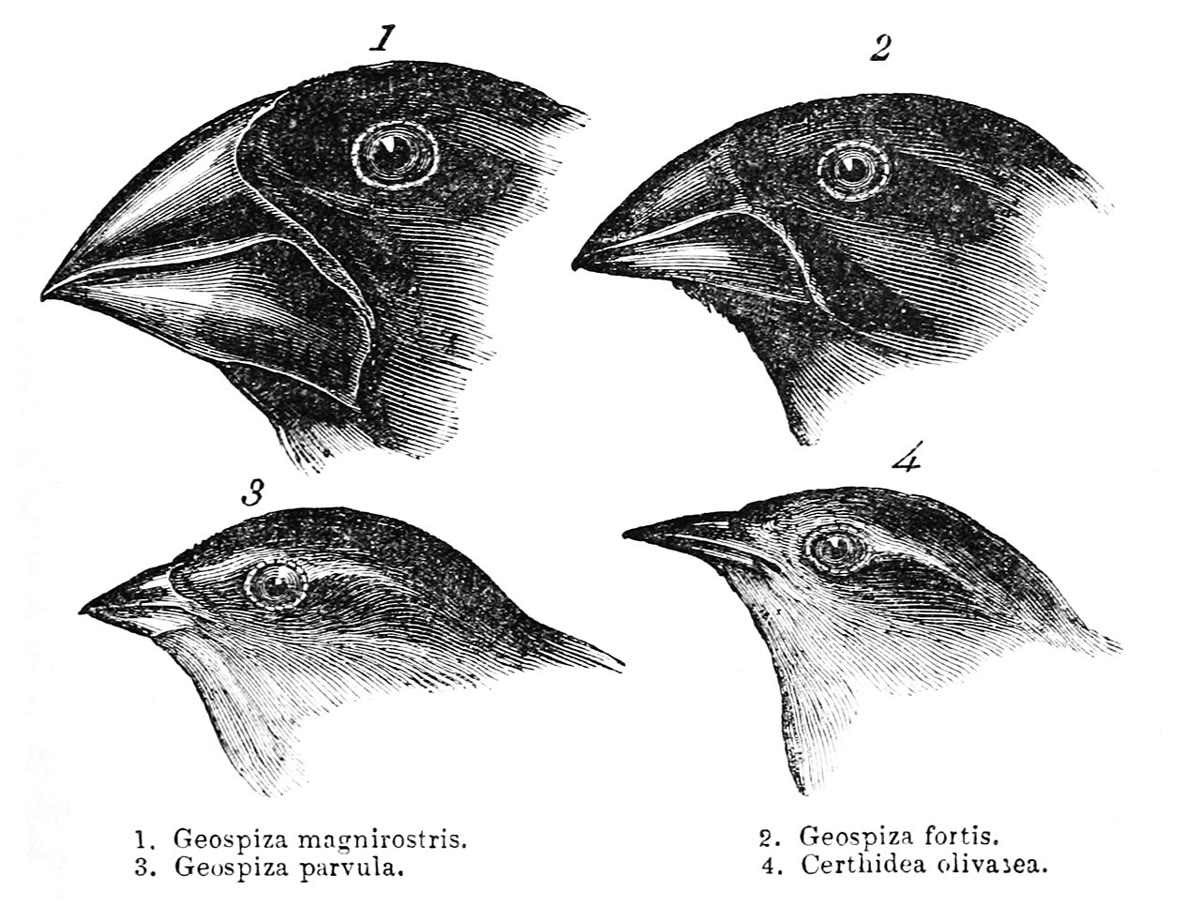
\includegraphics[width=0.62\linewidth]{images/book2/finches-gould.jpg}

{\small 达尔文雀中的四种，由约翰·古尔德于 1845 年依据\emph{贝格尔号}带回的标本绘制：除喙外其余一切相同，喙从胡桃夹到细针不等。一种生长信号在胚胎中剂量不同，便将它们区分开。雕版画，公有领域。}
\end{omfigure}

\section{共同生活：共生}

\begin{definition}[共生]\label{def:g12:diversification-of-life:symbiosis}
\emph{共生}\index{共生}是两个\omterm{def:g10:biodiversity-scales:species}{物种}之间持久而紧密的结合，
双方都从中获益。地衣是内含藻类\omterm{def:g10:cells-common-unit:cell}{细胞}的真菌，
藻类借\omterm{def:g10:cell-metabolism:autotrophy}{光合作用}为其提供养分，真菌则庇护并供水；
珊瑚是一种动物，其组织内含藻类；
多数植物的根被真菌包裹，真菌以矿物质换取糖分；
动物的肠道中则栖居着细菌，分解动物自身无法消化的物质。
这种结合能产生生物体、结构与生活方式，
而任何一方单独都无法达成。
\end{definition}

\begin{omfigure}
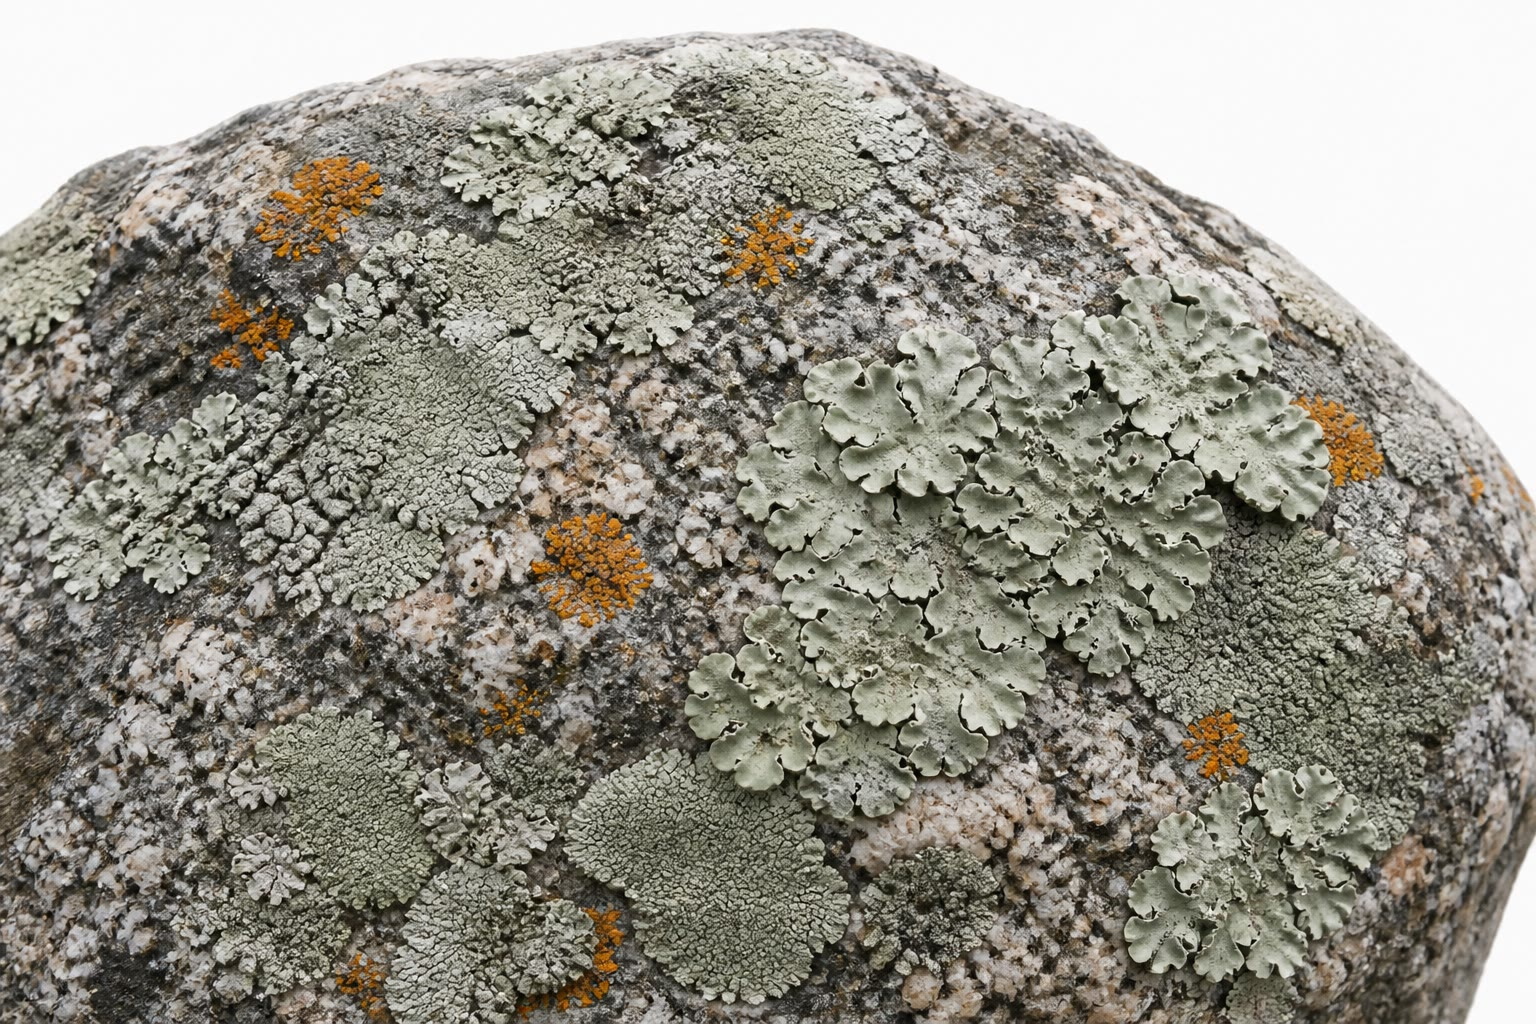
\includegraphics[width=0.58\linewidth]{images/book2/ai/g12-diversif-lichen.jpg}

{\small 花岗岩巨石上的地衣。每一块斑块都是真菌与一种藻类
融合而成的一个整体：一种能在裸岩上定殖、
任何一方都无法单独实现的生命形式。}
\end{omfigure}

\begin{proposition}[细胞内的共生]\label{prop:g12:diversification-of-life:endosymbiosis}
每个\omterm{def:g10:cells-common-unit:prokaryote}{真核细胞}的\omterm{def:g10:cells-common-unit:organelle}{线粒体}，以及植物\omterm{def:g10:cells-common-unit:cell}{细胞}的\omterm{def:g10:cells-common-unit:organelle}{叶绿体}，
均源自自由生活的细菌。这些细菌曾被吞入
一个祖先\omterm{def:g10:cells-common-unit:cell}{细胞}之中，约二十亿年前，并留存了下来。\omterm{def:g10:cells-common-unit:prokaryote}{真核细胞}本身
就是\omterm{def:g12:diversification-of-life:symbiosis}{共生}的产物。
\end{proposition}
\begin{proof}[证据]
\omterm{def:g10:cells-common-unit:organelle}{线粒体}和\omterm{def:g10:cells-common-unit:organelle}{叶绿体}有各自的 \omterm{def:g10:universal-dna:information}{DNA}，为小环状，与细菌的相似，
并有自己的\omterm{def:g10:cells-common-unit:organelle}{核糖体}，属于细菌类型，对
能阻断细菌\omterm{def:g10:cells-common-unit:organelle}{核糖体}而不阻断真核\omterm{def:g10:cells-common-unit:organelle}{核糖体}的\omterm{def:g11:antibiotic-resistance:antibiotic}{抗生素}敏感；
它们以一分为二的方式增殖，且不能由\omterm{def:g10:cells-common-unit:cell}{细胞}从头产生；
它们被两层膜包裹，内层膜类似
细菌的膜；就序列而言，它们的\omterm{def:g10:universal-dna:gene}{基因}与
某些特定类群的细菌最相近——\omterm{def:g10:cells-common-unit:organelle}{线粒体}对应紫色细菌，
\omterm{def:g10:cells-common-unit:organelle}{叶绿体}对应蓝细菌。
\end{proof}

\begin{omfigure}
\begin{tikzpicture}[font=\small, >=Stealth]
  % step 1: large cell + bacterium
  \draw[thick, fill=omDef!8] (0,0) ellipse (1.5 and 1.1);
  \draw[thick, fill=omDef!25] (-0.2,0.1) circle (0.4);
  \draw[thick, fill=omProp!40, rounded corners=4pt] (2.1,-0.15) rectangle (2.9,0.15);
  \node[anchor=north, align=center] at (0,-1.3) {祖先细胞 \\ 带细胞核};
  \node[anchor=north, align=center] at (2.5,-0.4) {进行呼吸的 \\ 细菌};
  \draw[->, thick] (3.6,0) -- (4.6,0) node[midway, above, font=\scriptsize] {被吞噬};
  % step 2: bacterium inside
  \begin{scope}[xshift=6.3cm]
    \draw[thick, fill=omDef!8] (0,0) ellipse (1.5 and 1.1);
    \draw[thick, fill=omDef!25] (-0.4,0.15) circle (0.4);
    \draw[thick, fill=omProp!40, rounded corners=4pt] (0.35,-0.5) rectangle (1.15,-0.2);
    \node[anchor=north, align=center] at (0,-1.3) {保留而未消化；\\ 在内部分裂};
  \end{scope}
  \draw[->, thick] (8.2,0) -- (9.2,0) node[midway, above, font=\scriptsize, align=center] {二十亿 \\ 年};
  % step 3: modern cell with mitochondria
  \begin{scope}[xshift=10.9cm]
    \draw[thick, fill=omDef!8] (0,0) ellipse (1.5 and 1.1);
    \draw[thick, fill=omDef!25] (-0.4,0.15) circle (0.4);
    \foreach \x/\y/\r in {0.5/0.4/20, 0.7/-0.3/-40, -0.2/-0.6/70}
      \draw[thick, fill=omProp!40, rotate around={\r:(\x,\y)}] (\x,\y) ellipse (0.3 and 0.13);
    \node[anchor=north, align=center] at (0,-1.3) {真核细胞：\\ 线粒体};
  \end{scope}
\end{tikzpicture}

{\small \omterm{def:g10:cells-common-unit:organelle}{线粒体}的起源。一个被祖先\omterm{def:g10:cells-common-unit:cell}{细胞}吞噬的细菌
被保留下来，并在其内增殖；其后代
是所有真核生物的\omterm{def:g10:cells-common-unit:organelle}{线粒体}，仍保留自身的
细菌型 \omterm{def:g10:universal-dna:information}{DNA} 和\omterm{def:g10:cells-common-unit:organelle}{核糖体}。\omterm{def:g10:cells-common-unit:organelle}{叶绿体}以同样方式
起源于一个光合细菌。}
\end{omfigure}

\section{无基因的多样性：行为}

\begin{proposition}[传递的行为]\label{prop:g12:diversification-of-life:behaviour}
在许多动物中，个体所做的部分事情是从
他者那里习得的——借助模仿、教导或复制——并依次传递：
一种\emph{文化}\index{文化（动物）}，不经由\omterm{def:g10:universal-dna:gene}{基因}传递。
同一\omterm{def:g10:biodiversity-scales:species}{物种}的种群之间，行为上也可以像\omterm{def:g10:universal-dna:gene}{等位基因}那样存在差异，
一种行为可在种群中扩散，
一代之内即可，而\omterm{def:g11:mutations:mutation}{突变}所需的则要经过许多代。
\end{proposition}
\begin{proof}[证据]
不同森林中的黑猩猩群体使用不同的工具——
这里用石头砸坚果，那里用木棍钓白蚁，别处则用树叶作
海绵——这些差异并不随遗传亲缘关系
或材料的可得性而变化；一只年幼的黑猩猩
通过观察长辈，学会本群体的这套工具。在隔离中饲养的鸣禽
唱的歌很粗糙；若能听到成鸟鸣叫，它们便唱
当地的方言，它随分布范围而变化，如同人的口音。一
群猕猴在一座岛上学会了在海中清洗红薯，
十年之内，由一只年轻雌猴带头学会，其后代至今仍然如此。
\end{proof}

\begin{omfigure}
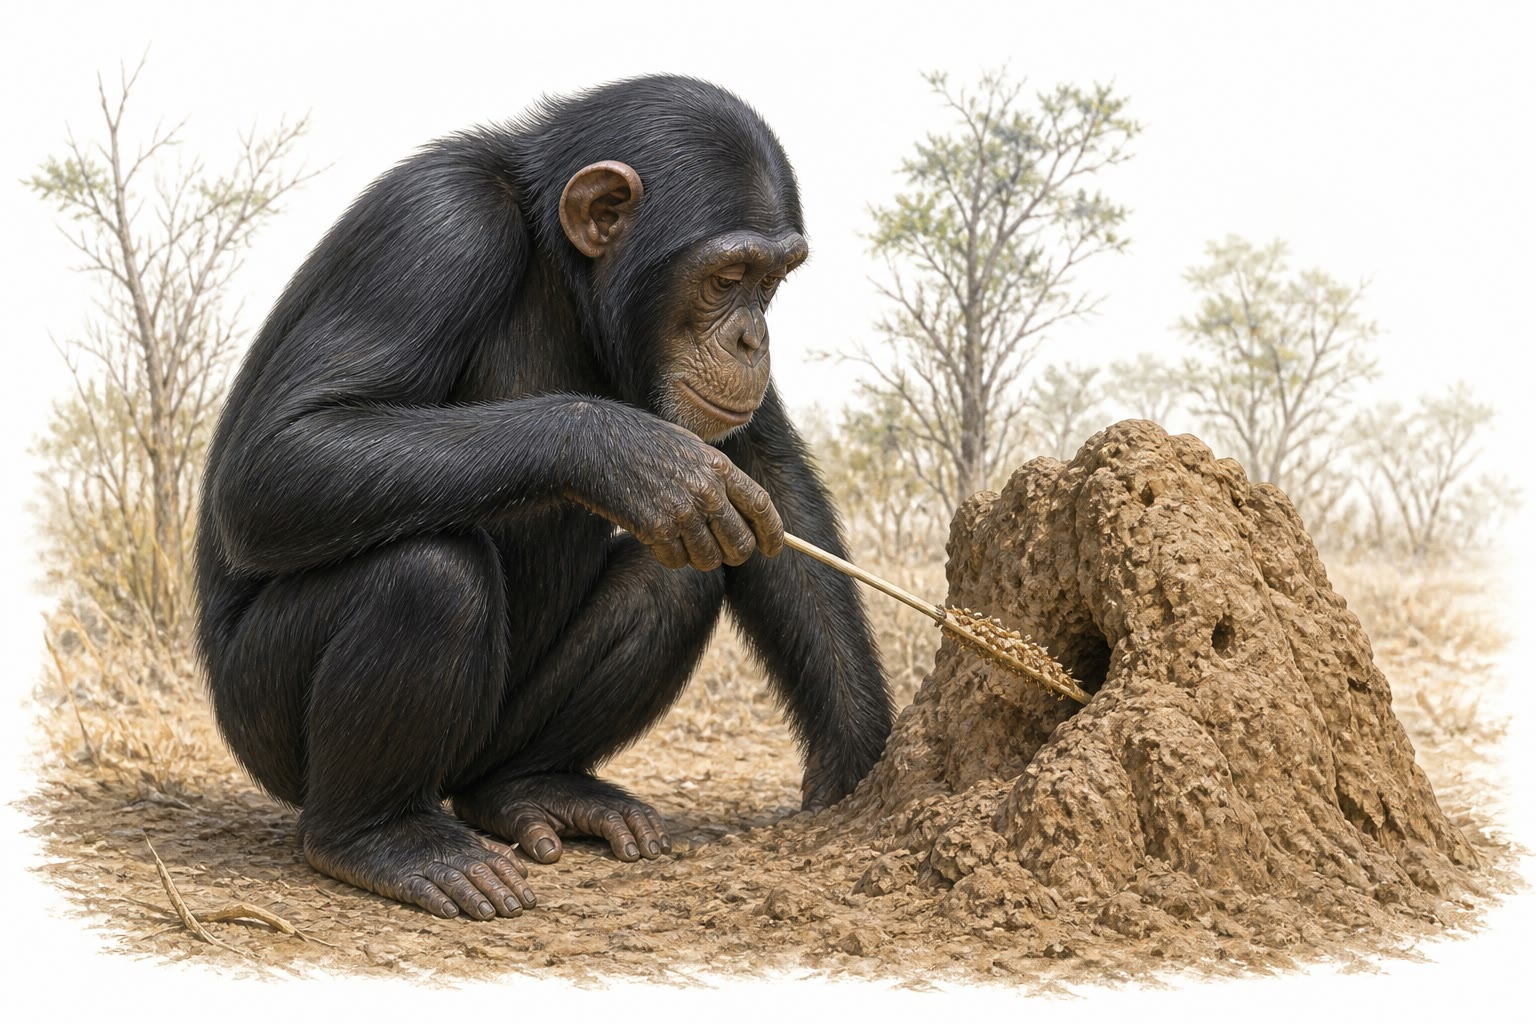
\includegraphics[width=0.6\linewidth]{images/book2/ai/g12-diversif-chimp-tool.jpg}

{\small 一只黑猩猩用削好的木棍钓白蚁。
这一技巧通过观察习得，且因群体而异，
即一种不经\omterm{def:g10:universal-dna:gene}{基因}传递的传统。}
\end{omfigure}

\begin{method}[命名差异的来源]\label{met:g12:diversification-of-life:name}
面对两个生物体或种群之间的差异：
\begin{enumerate}
  \item 差异是否出现在\omterm{def:g10:universal-dna:gene}{基因}序列中（\omterm{def:g11:mutations:mutation}{突变}、\omterm{def:g10:universal-dna:gene}{等位基因}）？
        是否出现在\omterm{def:g10:universal-dna:gene}{基因}拷贝数中（重复）？是否出现在
        来自他处的\omterm{def:g10:universal-dna:gene}{基因}之中（水平转移）？是否出现在
        \omterm{def:g11:cell-cycle-mitosis:chromosome}{染色体}组数中（\omterm{prop:g12:diversification-of-life:polyploidy}{多倍体}）？
  \item 差异是否在于一个共有\omterm{def:g10:universal-dna:gene}{基因}在
        发育中何时、何处或表达多少（调控）？
  \item 差异是否源于与另一\omterm{def:g10:biodiversity-scales:species}{物种}建立关联的结果
        （\omterm{def:g12:diversification-of-life:symbiosis}{共生}）？
  \item 差异是否为习得的（经文化传递的行为）——可遗传，
        但非\omterm{def:g10:universal-dna:gene}{基因}遗传？
\end{enumerate}
往往不止一个答案正确；这些问题构成
本章内容的清单。
\end{method}

\begin{remark}[多样化与选择]\label{rem:g12:diversification-of-life:selection}
这里的每一过程都产生变异；没有一个能决定
何者得以存续。\omterm{prop:g12:diversification-of-life:polyploidy}{多倍体}小麦、蟒蛇的表达模式、地衣，
砸坚果的传统，各自得以延续，因为它们在
出现之地行之有效。变异的筛选——即选择与机遇——是
下一章的主题；本章已阐明有多少变异可供筛选，
以及有多少种产生它的方式。
\end{remark}

\section{练习}

\begin{exercise}[$\star$]\label{exo:g12:diversification-of-life:1}
列出除点\omterm{def:g11:mutations:mutation}{突变}之外的五种多样化来源。
\end{exercise}

\begin{exercise}[$\star$]\label{exo:g12:diversification-of-life:2}
什么是\omterm{prop:g12:diversification-of-life:duplication}{基因家族}？它是如何产生的？
\end{exercise}

\begin{exercise}[$\star$]\label{exo:g12:diversification-of-life:3}
为什么两个\omterm{def:g10:biodiversity-scales:species}{物种}之间的杂种通常不育，
\omterm{def:g11:cell-cycle-mitosis:chromosome}{染色体}加倍如何使其恢复可育？
\end{exercise}

\begin{exercise}[$\star$]\label{exo:g12:diversification-of-life:4}
给出\omterm{def:g10:cells-common-unit:organelle}{线粒体}起源于细菌的三条证据。
\end{exercise}

\begin{exercise}[$\star$]\label{exo:g12:diversification-of-life:5}
什么是动物中的文化？请举一例。
\end{exercise}

\begin{exercise}[$\star\star$]\label{exo:g12:diversification-of-life:6}
二粒小麦的 $2n = 28$，一粒小麦的 $2n = 14$；它们的杂种有多少条\omterm{def:g11:cell-cycle-mitosis:chromosome}{染色体}，
\omterm{def:g12:meiosis-genetic-shuffling:meiosis}{减数分裂}时能形成多少对？试解释
其不育的原因。
\end{exercise}

\begin{exercise}[$\star\star$]\label{exo:g12:diversification-of-life:7}
$\alpha$ 与 $\beta$ 珠蛋白\omterm{def:g10:universal-dna:gene}{基因}的相同率为 50\%；$\beta$
与 $\gamma$ \omterm{def:g10:universal-dna:gene}{基因}的相同率为 80\%。哪一次\omterm{def:g10:universal-dna:gene}{基因}重复更古老？画出系统树。
\end{exercise}

\begin{exercise}[$\star\star$]\label{exo:g12:diversification-of-life:8}
试解释蟒蛇为何没有腿，尽管它携带着
蜥蜴中构建腿的那些\omterm{def:g10:universal-dna:gene}{基因}。
\end{exercise}

\begin{exercise}[$\star\star$]\label{exo:g12:diversification-of-life:9}
两种雀鸟的喙深相差两倍，而
其喙\omterm{def:g10:universal-dna:gene}{基因}却完全相同。差异在哪里？为什么它能
迅速产生？
\end{exercise}

\begin{exercise}[$\star\star$]\label{exo:g12:diversification-of-life:10}
仅由其真菌单独培养出的，是一团无定形的霉菌；仅由其藻类
单独培养出的，则是一层绿膜。试解释地衣在何种意义上是一种
新型生物。
\end{exercise}

\begin{exercise}[$\star\star$]\label{exo:g12:diversification-of-life:11}
一个黑猩猩种群会敲开坚果；隔着一条河的邻近种群
则不会，尽管两岸都有大量坚果和石块。
利用\cref{met:g12:diversification-of-life:name}，
判断差异的来源并给出理由。
\end{exercise}

\begin{exercise}[$\star\star\star$]\label{exo:g12:diversification-of-life:12}
人类\omterm{def:g10:universal-dna:gene}{基因}组中的一个\omterm{def:g10:universal-dna:gene}{基因}，与某种病毒的\omterm{def:g10:universal-dna:gene}{基因}几乎相同，
而在灵长类以外的任何哺乳动物中找不到与之相似的\omterm{def:g10:universal-dna:gene}{基因}。提出它的
历史，并说明如何检验这一假设。
\end{exercise}

\begin{exercise}[$\star\star\star$]\label{exo:g12:diversification-of-life:13}
阻断细菌\omterm{def:g10:cells-common-unit:organelle}{核糖体}的\omterm{def:g11:antibiotic-resistance:antibiotic}{抗生素}，在高剂量下会对患者的
\omterm{def:g10:cells-common-unit:organelle}{线粒体}产生副作用。试解释原因，并说明这一点
对\omterm{def:g10:cells-common-unit:organelle}{线粒体}的祖先来源有何启示。
\end{exercise}

\begin{exercise}[$\star\star\star$]\label{exo:g12:diversification-of-life:14}
试解释为何新的\omterm{prop:g12:diversification-of-life:polyploidy}{多倍体}\omterm{def:g10:biodiversity-scales:species}{物种}从第一代起就与其亲本
产生生殖隔离，而一个新\omterm{def:g10:universal-dna:gene}{等位基因}需要多代才能
扩散开来。由此推测，植物\omterm{def:g10:biodiversity-scales:species}{物种}可以多快
形成？
\end{exercise}

\begin{exercise}[$\star\star\star$]\label{exo:g12:diversification-of-life:15}
“一切多样性都来自\omterm{def:g11:mutations:mutation}{突变}。”请用一段文字讨论：这一说法
在何种意义上从根本上是对的，本章所述的过程又在哪些方面
超越了它。
\end{exercise}

\section{问题：面包中的三种禾草}

\begin{problem}[{周末问题——由染色体重建面包小麦的历史，把
蟒蛇的基因与小鼠的基因并排比较，并让每个细胞内的
细菌接受审判}]
\label{pb:g12:diversification-of-life:1}
一粒小麦（AA）、山羊草 1（BB）和山羊草 2（DD）各自
均有 $2n = 14$。二粒小麦为 AABB，面包小麦为 AABBDD。

\medskip
\noindent\textbf{第一部分——小麦的\omterm{def:g11:cell-cycle-mitosis:chromosome}{染色体}。}
\begin{enumerate}
  \item 给出二粒小麦和面包小麦的\omterm{def:g11:cell-cycle-mitosis:chromosome}{染色体}数目。
  \item 一粒小麦与山羊草 1 的杂种有 14 条\omterm{def:g11:cell-cycle-mitosis:chromosome}{染色体}，
        每种各 7 条。\omterm{def:g12:meiosis-genetic-shuffling:meiosis}{减数分裂}时能形成多少对\omterm{def:g10:common-ancestry:homology}{同源}\omterm{def:g11:cell-cycle-mitosis:chromosome}{染色体}？
        其配子情况如何？
  \item 试解释\omterm{def:g11:cell-cycle-mitosis:chromosome}{染色体}加倍为何能恢复可育性：
        数出其中的对数。
  \item 二粒小麦与山羊草 2 的杂种有 21 条\omterm{def:g11:cell-cycle-mitosis:chromosome}{染色体}。其中哪些
        能够配对？它为何不育？
  \item 加倍后，面包小麦有 42 条\omterm{def:g11:cell-cycle-mitosis:chromosome}{染色体}。\omterm{def:g12:meiosis-genetic-shuffling:meiosis}{减数分裂}时能形成多少对，
        且一个花粉粒携带多少条\omterm{def:g11:cell-cycle-mitosis:chromosome}{染色体}？
\end{enumerate}

\medskip
\noindent\textbf{第二部分——解读历史。}
\begin{enumerate}[resume]
  \item 面包小麦多数\omterm{def:g10:universal-dna:gene}{基因}有三个拷贝，分别位于每一组
        \omterm{def:g11:cell-cycle-mitosis:chromosome}{染色体}组上。解释为何一个拷贝被\omterm{def:g11:mutations:mutation}{突变}破坏通常不产生可见效应，以及
        这一点在长期进化中允许什么。
  \item 二粒小麦约于 10\,000 年前已被栽培，面包小麦在考古遗址中
        出现于 8\,000 年前。第二次杂交最可能在何时何地发生？
        又需要哪些植物
        并排生长？
  \item 将二粒小麦与山羊草 2 进行实验室杂交，
        再经化学加倍，得到与面包小麦相似的可育植株。
        这证实了上述历史中的哪一项结论？
  \item 面包小麦与一粒小麦杂交无法产生可育后代，
        它是否为独立\omterm{def:g10:biodiversity-scales:species}{物种}？请利用
        \cref{ch:g10:biodiversity-scales}中的定义加以论证。
  \item 一位作物育种者希望将一个抗病\omterm{def:g10:universal-dna:gene}{基因}
        从山羊草 2 导入面包小麦。试解释为何这比从
        无亲缘关系的植物中导入更容易。
\end{enumerate}

\medskip
\noindent\textbf{第三部分——蟒蛇的\omterm{def:g10:universal-dna:gene}{基因}。}
\begin{enumerate}[resume]
  \item 小鼠与蟒蛇的躯干区域\omterm{def:g10:universal-dna:gene}{基因}相同率为 98\%。这
        表明两者身体差异的来源
        在哪里？
  \item 小鼠胚胎中，“有肋躯干”\omterm{def:g10:universal-dna:gene}{基因}活跃于 13
        个体节；蟒蛇中则约在 300 个体节上活跃。
        请指出所涉及的变化类型。
  \item 蟒蛇胚胎在后肢本应存在的位置形成微小的芽，
        随后便停止生长。这提示我们，关于肢体\omterm{def:g10:universal-dna:gene}{基因}
        及激活它们的信号，可以得出什么结论？
  \item 经改造、在腰部表达“有肋躯干”\omterm{def:g10:universal-dna:gene}{基因}的小鼠，
        在该处长出额外的肋骨。这一实验
        为这一比较增添了什么？
  \item 比较两类变化：面包小麦的与蟒蛇的，
        哪一类改变了\omterm{def:g10:universal-dna:gene}{基因}组的大小，哪一类改变了\omterm{def:g10:universal-dna:gene}{基因}的用途？
\end{enumerate}

\medskip
\noindent\textbf{第四部分——体内的细菌。}
\begin{enumerate}[resume]
  \item 列出四个符合细菌起源的\omterm{def:g10:cells-common-unit:organelle}{线粒体}特征，
        并对每一特征说明，若\omterm{def:g10:cells-common-unit:organelle}{线粒体}是由\omterm{def:g10:cells-common-unit:cell}{细胞}从头构建的，
        应当会有怎样的情况？
  \item \omterm{def:g10:cells-common-unit:organelle}{线粒体} \omterm{def:g10:universal-dna:information}{DNA} 只携带 37 个\omterm{def:g10:universal-dna:gene}{基因}，而\omterm{def:g10:cells-common-unit:organelle}{线粒体}约需 1500
        种\omterm{def:g11:gene-expression:protein}{蛋白质}。其余\omterm{def:g10:universal-dna:gene}{基因}在哪里？
        它们在二十亿年间发生了什么？
  \item 人体的每个\omterm{def:g10:cells-common-unit:organelle}{线粒体}都来自卵\omterm{def:g10:cells-common-unit:cell}{细胞}，
        没有一个来自精子。这对\omterm{def:g10:cells-common-unit:organelle}{线粒体}\omterm{def:g10:universal-dna:gene}{基因}的遗传，以及
        追溯母系祖先，有什么推论？
  \item 地衣与\omterm{def:g10:cells-common-unit:organelle}{线粒体}都属于\omterm{def:g12:diversification-of-life:symbiosis}{共生}。\omterm{def:g10:cells-common-unit:organelle}{线粒体}的\omterm{def:g12:diversification-of-life:symbiosis}{共生}
        在哪一方面走得更远？
  \item 请给出结论：面包中的三个\omterm{def:g10:biodiversity-scales:species}{物种}，及各自贡献的
        \omterm{def:g11:cell-cycle-mitosis:chromosome}{染色体}数目；用一个词指出蟒蛇与小鼠在使用共有\omterm{def:g10:universal-dna:gene}{基因}
        方面的差异；
        以及哪一种\omterm{def:g10:cells-common-unit:organelle}{细胞器}曾是一种细菌。
\end{enumerate}
\end{problem}
